\documentclass{beamer}

%-------



\usepackage{amsthm}
\usepackage{amsmath}
\usepackage{natbib}
\bibliographystyle{apalike}
\usepackage{graphicx, psfrag, amsfonts, float}
\usepackage{natbib}
\usepackage{amsthm}
\usepackage{multirow}
\usepackage{hhline}
\usepackage{rotating}
\def\bgam{\mbox{\boldmath $\gamma$}}
\def\bth{\mbox{\boldmath $\theta$}}
\def\bbeta{\mbox{\boldmath $\beta$}}
\def\blam{\mbox{\boldmath $\lambda$}}
\def\bmu{\mbox{\boldmath $\mu$}}

\newcommand{\bx}{\mbox{\boldmath $x$}}
\newcommand{\bu}{\mbox{\boldmath $u$}}
\newcommand{\bc}{\mbox{\boldmath $c$}}
\newcommand{\bs}{\mbox{\boldmath $s$}}
\newcommand{\by}{\mbox{\boldmath $y$}}
\newcommand{\bz}{\mbox{\boldmath $z$}}
\newcommand{\bv}{\mbox{\boldmath $v$}}
\newcommand{\bb}{\mbox{\boldmath $b$}}
\newcommand{\bzero}{\mbox{\boldmath $0$}}
\newcommand{\thstarj}{\mbox{$\theta^\star_j$}}
\newcommand{\bths}{\mbox{$\btheta^\star$}}
\newcommand{\pkg}[1]{{\fontseries{b}\selectfont #1}} 

\newcommand{\ud}{\mathrm{d}}
\newcommand{\uI}{\mathrm{I}}
\newcommand{\uP}{\mathrm{P}}
\newcommand{\up}{\mathrm{p}}
\newcommand{\mb}{\mathbf}
\newcommand{\mc}{\mathcal}


\newcommand{\Bern}{\mbox{Bern}}
\newcommand{\Nor}{\mbox{N}}
\newcommand{\Ga}{\mbox{Gamma}}
\newcommand{\Dir}{\mbox{Dir}}
\newcommand{\Ber}{\mbox{Ber}}
\newcommand{\Be}{\mbox{Be}}
\newcommand{\Unif}{\mbox{Unif}}
\newcommand{\Binom}{\mbox{Bin}}
\newcommand{\IG}{\mbox{IG}}

\newcommand{\Xs}{X^\star}
\newcommand{\Lc}{{\cal L}}



\newcommand{\iid}{\stackrel{iid}{\sim}}
\newcommand{\indep}{\stackrel{indep}{\sim}}


% commands for for editing
\usepackage{color}
\usepackage{ulem} % \sout
\newcommand{\red}[1]{{\color{red}#1}}
\newcommand{\blue}[1]{{\color{blue}#1}}
\newcommand{\brown}[1]{{\color{brown}#1}}
\newcommand{\green}[1]{{\color{green}#1}}
\newcommand{\magenta}[1]{{\color{magenta}#1}}
\newcommand{\response}[1]{{\color{blue}#1}}
\DeclareMathOperator*{\argmin}{\arg\!\min}
\graphicspath{{figures_final/}}


%-------



%Information to be included in the title page:
%Information to be included in the title page:
\title{Bayesian Restricted Likelihood Methods: Conditioning on Insufficient Statistics in Bayesian Regression}

\author{John R. Lewis \and Steven N. MacEachern \and Yoonkyung Lee}
\institute{Department of Statistics, The Ohio State University}
\date{Feb. 9, 2022}


\begin{document}
	
%\frame{\titlepage}

%\begin{frame}
%\frametitle{Introduction}
%
%\begin{itemize}
%\item Formal Bayesian inference relies on the prior, likelihood, loss
%\item Each require assumptions that should be questioned
%\item We focus this paper on imperfections in the Likeihood:
%
%\begin{itemize}
%\item Start with a full model as if it is correct
%
%\item Sumarise the data with a summary statistic
%
%\item The prior is updated with the summary statistic rather than the complete data
%\end{itemize}
%\end{itemize}
%\end{frame}
%	
%
%\begin{frame}
%\frametitle{Resticted Likelihood Examples}
%
%\begin{itemize}
%	\item Outliers
%\begin{itemize}
%	\item Known subset of bad data are removed prior to analysis. 
%\end{itemize}
%\begin{eqnarray*}
%	\label{OutlyingCases}
%	L(\bth | \by)  
%	= \left( \prod_{i=1}^{n-k} f(y_i | \bth) \right) \left( \prod_{i=n-k+1}^{n} f(y_i | \bth) \right) 
%\end{eqnarray*}
%\end{itemize}
%\end{frame}
%
%\begin{frame}
%\frametitle{Resticted Likelihood Examples}
%
%\begin{itemize}
%	\item Censoring 
%\begin{itemize}
%		\item Reaction Time Experiments \citep[e.g.,][]{ratcliff1993}
%		\item Some reactions are too fast or too slow to be believable
%\end{itemize}
%\item $c(y_i)= t_1$ if $y_i \leq t_1$, $c(y_i)=t_2$ 
%if $y_i \geq t_2$, and $c(y_i)=y_i$ otherwise.
%\begin{eqnarray*}
%\label{Censoring} 
%L(\bth  | \by) =  \left( \prod_{i=1}^n g(c(y_i)  | \bth) \right) \left( \prod_{i=1}^n f(y_i|\bth,c(y_i)). \right) 
%\end{eqnarray*}
%\end{itemize}
%
%\end{frame}
%
%
%
%\begin{frame}
%\frametitle{Resticted Likelihood Generalization}
%\begin{itemize}
%	\item Conditioning statistic $T(\by)$
%	\begin{itemize}
%		\item Example 1: $T(\by) = (y_1, \ldots, y_{n-k})$
%		\item Example 2: $T(\by) = (c(y_1),\ldots,c(y_n))$
%	\end{itemize}
%\begin{eqnarray*}
%\label{FullLikelihood}
%L(\bth | \by)  
%& = & f(T(\by) | \bth) \,\, f(\by |\bth, T(\by)) 
%\end{eqnarray*}
%\item Restricted Likelihood Posterior
%\begin{eqnarray*}
%\label{RestrictedPosterior}
%\pi(\bth | T(\by)) & = & \frac{\pi(\bth) f(T(\by) | \bth)}{m(T(\by))} 
%\end{eqnarray*}
%
%\item Predictive Density 
%\begin{eqnarray*}
%\label{RestrictedpredDist}
%f(y_{n+1} | T(\by)) = \int f(y_{n+1} | \bth) \pi(\bth | T(\by))\ d\bth 
%\end{eqnarray*}
%\end{itemize}
%
%
%
%\end{frame}
%
%\begin{frame}
%\frametitle{Literature Review}
%\begin{itemize}
%	\item Rank Likelihoods: \cite{savage1969}, \cite{pettitt1983, pettitt1982}, \cite{hoff2013}.  
%	\item Order Statistics: \cite{lewis2012}
%	\item Asymptotics: \cite{doksum1990}, \cite{clarke1995}, \cite{yuan2004},  and \cite{hwang2005}
%	\begin{itemize}
%		\item Often, posterior distribution resembles the asymptotic sampling distribution of the conditioning statistic
%	\end{itemize}
%	\item Approximate sufficiency of mean/sd: \cite{pratt1965}
%\end{itemize}
%\end{frame}
%
%
%\begin{frame}
%\frametitle{Literature Review: Approximate Bayesian Computation}
%\begin{itemize}
%	\item Posterior approximation with success in many applications: \citep{tavare1997, pritchard1999, beaumont2002, marjoram2003, fearnhead2012, drovandi2015}.
%	\item $L(\bth| \mathcal{B}(\by))$, where $\mathcal{B}(\by)=\{\by^{*}|\rho(T(\by),T(\by^{*})) \leq \epsilon\}$
%	\begin{itemize}
%	\item metric $\rho$, tolerance level $\epsilon$
%\end{itemize}
%\item Goal is often to approximate the full posterior
%\item Choose an approximately sufficient \citep{joyce2008} $T(\by)$ and small $\epsilon$
%\item Sampling Methods: Standard reject \citep{pritchard1999}, Extensions: \cite{beaumont2009, turner2012, turner2014}
%\end{itemize}
%\end{frame}


\begin{frame}
\frametitle{Application to the Linear Model}
\begin{eqnarray*}
	\label{LinearModel}
	\bth&=&(\bbeta,\sigma^2) \sim  \pi(\bth) 
	\nonumber\\
	y_i  & =  & x_i^\top \bbeta + \epsilon_i , \mbox{ for } i = 1, \ldots, n 
\end{eqnarray*}

\begin{itemize}
	\item $T(\by) = (\bb(X, \by), s(X, \by))$ 
\begin{itemize}
	\item $\bb(X, \by)= (b_1(X,\by), \dots,b_p(X,\by))^\top\in \mathbb R^{p}$ 
	\item $s(X, \by)\in \{0\} \cup {\mathbb R}^+$
\end{itemize}
	\item E.g. M-estimators \cite{huber1964}, Least Median Squares, Least Trimmed Squares 
\end{itemize}


\end{frame}

\begin{frame}
\frametitle{Computational Strategy}
\begin{itemize}
	\item Numerical integration (low dimension), Appeal to asymptotics.
	\item MCMC: Data augmented Gibbs Sampler targeting $f(\bth, \by | T(\by)=T(\by_{obs}))$
	\begin{enumerate}
		\item $\pi(\bth|\by, T(\by)=T(\by_{obs})) = \pi(\bth | \by)$ (full poserior)
		\item $f(\by|\bth, T(\by)=T(\by_{obs}))$ 
	\end{enumerate}
\item For 2, prosose a Metropolis-Hastings sampler.
\item accept/reject a sample full data $\by \in \mathcal{A}:=\{\by \in \mathbb{R}^n | T(\by)=T(\by_{obs})\}$ from a well defined distribution with support  $\mathcal{A}$.
\end{itemize}
	
\end{frame}

\begin{frame}
	\frametitle{Computational Strategy}
	\begin{itemize}
		\item Difficult to sample from $ \mathcal{A}$ directly
		\item Can sample $\bz^{*} \in \mathbb{R}^{n}$ and transform:
		$$\by = h(\bz^*) := \frac{s(X,\by_{obs})}{s(X,\bz^*)} \bz^* + X\left(\bb(X,\by_{obs}) - \bb(X,\frac{s(X,\by_{obs})}{s(X,\bz^*)} \bz^*)\right) $$
		\item With regression/scale equivariance/invariance properties (C3-C8 in the paper) $T(y) = T(y_{obs})$
		\item Idea: 
		\begin{itemize}
		\item sample $\bz^{*}\sim p(\bz^*)$, transform via $h$
		\item proposal $p(\by|\bth)$ is then a change-of-variables adjustment on $p(\bz^*)$.
	\end{itemize}
	\end{itemize}	
\end{frame}


\begin{frame}
	\frametitle{Computational Strategy}
	\begin{itemize}
	\item $h$ is not 1-1/onto. (Change of variables difficult)
	\item Can restrict sample space of $z^{*}$, so that it is
	\begin{itemize}
		\item $\mathcal{A}$ is an $n - p - 1$ space
		\item Sample space for $z^{*}$:  $\mathbb{S} := \{\bz^* \in \mathcal{C}^{\perp}(X)\  |\  ||\bz^*|| = 1\}$
		\begin{itemize}
			\item i.e. the unit space in the orthogonal complement of the column space of the design matrix.
		\end{itemize}
	\item $h: \mathbb{S} \rightarrow \mathcal{A}$ is then 1-1/onto.
	\item easier to figure out the Jacobian of the transformation from  $p(\bz^*)$ to $p(\by|\bth)$
	\end{itemize}
	
	\end{itemize}	
\end{frame}

\begin{frame}
	\frametitle{Computational Strategy}
	For the proposal distribution. 
	\begin{enumerate}
		\item Sample $\bz^*$ from a distribution with known density with support $\mathbb{S}$.
		\item Set $\by = h(\bz^*)$
		\item Jacobian broken into steps
	\begin{itemize}
		\item $\bz=\frac{s(X,\boldsymbol{y}_{obs})}{s(X, \boldsymbol{z}^{*})}\bz^{*}$. 
		\begin{itemize}
			\item Scale from $\mathbb{S}$ to the set $\Pi(\mathcal{A}):= \{\bz\in \mathbb{R}^n |\ \exists\ \by\in \mathcal{A}\ s.t.\ \bz=Q \by \}$ with $Q = I - XX^{\top}$.
	\end{itemize}
		\item $\by=\bz+X\left(\bb(X, \by_{obs})-\bb(X, \bz)\right)$. 
	\begin{itemize}
		\item Shift from $\Pi(\mathcal{A})$ to $\mathcal{A}$ along $\mathcal{C}(X)$
	\end{itemize}
	\end{itemize}
	\end{enumerate}
\end{frame}

\begin{frame}
	\frametitle{Computational Strategy (Visualization, $n=3, p=1$)}
$T(\by)=(\min(\by),\sum (y_i - \min(\by))^2)$, $T(\by_{obs})=(0,1)$
\begin{figure}[t]
	\centering
	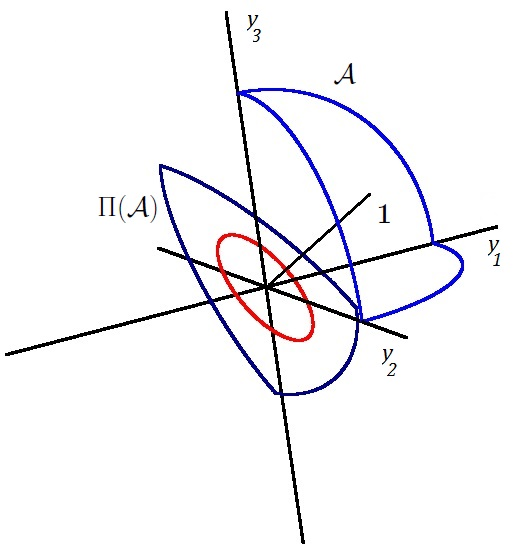
\includegraphics[width=2.5in]{minSS3dSampleSpace.jpg}
	\label{fig:sampSpace}
\end{figure}
	
\end{frame}


\begin{frame}
	\frametitle{Computational Strategy (Visualization, $n=3, p=1$)}
Scaling step
\begin{figure}[t]
		\centering
		{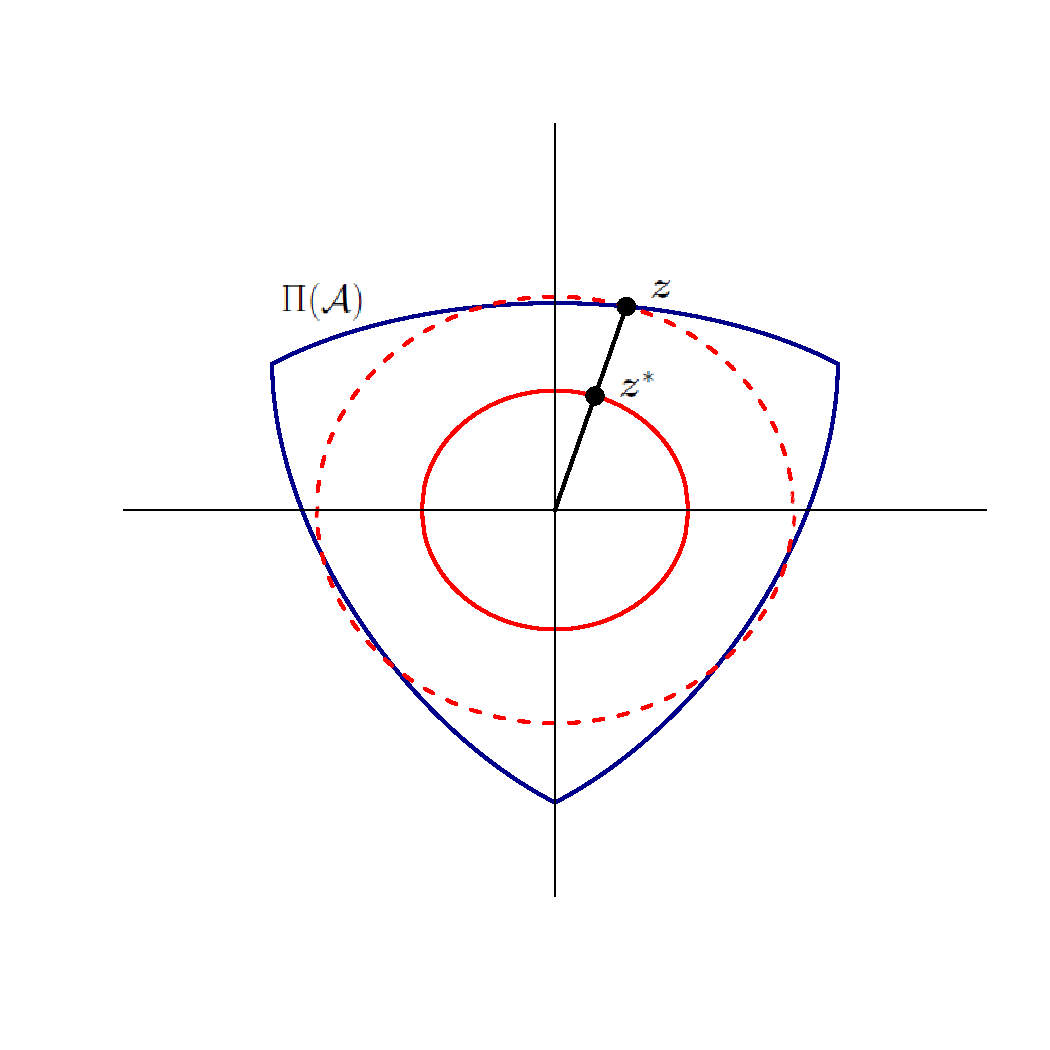
\includegraphics[width=2in]{minSSZSpace3.pdf}}
		{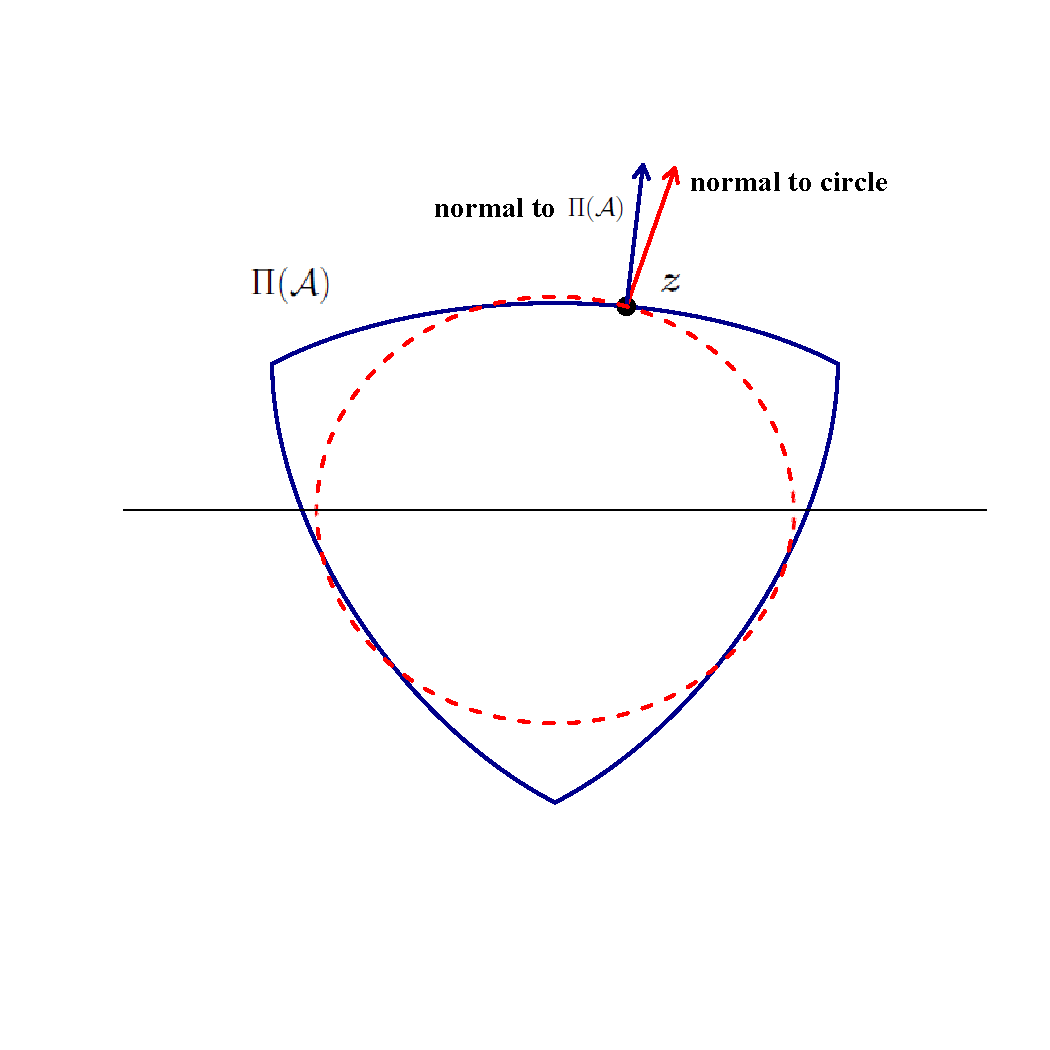
\includegraphics[width=2in]{minSSZSpace5.pdf}}
		\label{fig:stretchDeform}
\end{figure}
\begin{itemize}
	\item resize sphere: $r^{-(n-p-1)}$
	\item deformation onto $\Pi(\mathcal{A}): \cos(\gamma)=\frac{\nabla s(X,\by)^\top \bz}{\|\nabla
		s(X,\by)\| \|\bz\|}$
\end{itemize}

\end{frame}


\begin{frame}
	\frametitle{Computational Strategy (Visualization, $n=3, p=1$)}
  	Shifting step of $\bz$ to $\by$ along the column space of $X$
	\begin{itemize}
		\item Contribution is the ratio of the infinitesimal volumes along $\Pi(\mathcal{A})$ at $\bz$ to the
		corresponding volume along $\mathcal{A}$ at $\by$. 
		\item $\text{Vol} (P) := \sqrt{\text{det}(P^\top P)}=\prod_{i=1}^{r} \sigma_i$
		\begin{itemize}
			\item $P = QA$, 
			\item columns of $A$: an orthonormal basis for the tangent
			space to $\mc A$ at $\by$. 
			\item $\nabla s(X,\by), \nabla b_1(X,\by),\dots, \nabla b_p(X,\by)$ form basis for the orthogonal complement.
			\item $\sigma_i$ are the singular values of $P$
		\end{itemize}
	Full Jacobian: $p(\by)=p(\bz^*) r^{-(n-p-1)} \cos(\gamma)\text{Vol} (P)$
	\end{itemize}
	
\end{frame}



%
%\begin{frame}
%\frametitle{Simulation Example 1}
%	\begin{itemize}
%		\item  hierarchical setting with outliers.
%	\end{itemize}
%\begin{align*}
%\label{gensim2}
%\begin{split}
%& \theta_{i}  \sim   N(0, 1),  \ i = 1, 2, \dots, 90  \\ 
%& y_{ij} \sim (1-p_{i})N(\theta_{i}, 4) + p_{i}N(\theta_{i}, 4m_{i}),\  j = 1, 2,..., n_{i}
%\end{split}
%\end{align*}
%\begin{itemize}
%	\item $p_{i} = .1, .2, .3$, $m_{i} = 9, 25$, and $n_{i} = 25, 50, 100$
%	\item 5 groups for each combination, 90 groups total
%	\item Base model for fitting:
%\end{itemize}
%\begin{equation*}
%\label{fullsim2}
%\begin{split}
%%& \mu \propto 1, \  \tau^{2} \propto \tau^{-2}, \\
%& \theta_{i}\sim N(\mu, \tau^{2}), \  \sigma^{2}_{i} \sim IG(a_{s}, b_{s}),  \ i = 1, 2, \dots, 90, \\ 
%& y_{ij}\sim  N(\theta_{i},\sigma^{2}_{i}), \ j = 1, 2, \dots, n_{i}.
%\end{split}
%\end{equation*}
%\begin{itemize}
%	\item Restricted likihood fit: Robust M-estimators for each group: $T_{i}(y_{i1}, \dots, y_{in_{i}}) = (\hat\theta_{i}, \hat\sigma^{2}_{i}), i = 1, 2, ..., 90$.
%\end{itemize}
%\end{frame}
%
%
%\begin{frame}
%	\frametitle{K = 30 simulations, M indexes the method, MSE}
%\begin{figure}[t]
%	\centering
%	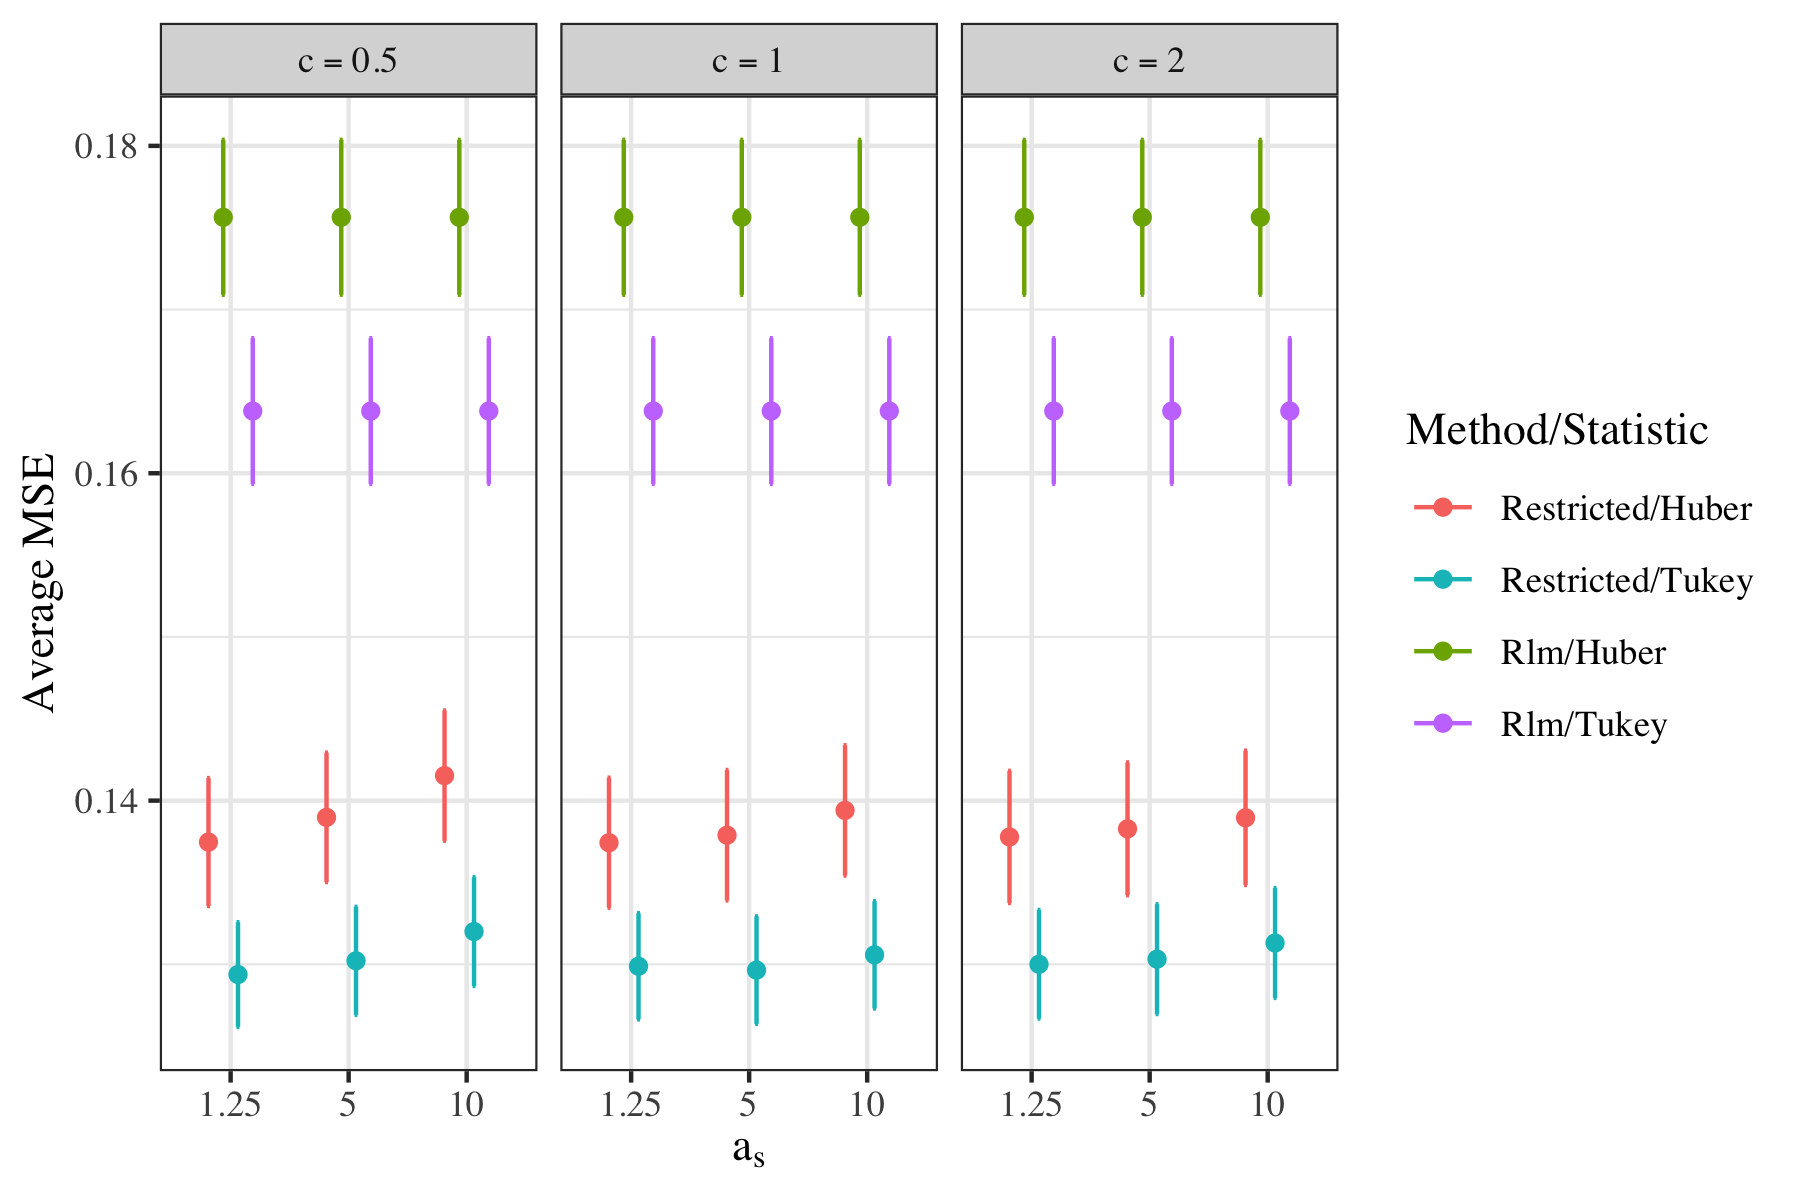
\includegraphics[width = 3.5in]{mse_sim2_facet_scale.png}
%	\caption{Average MSE plus/minus one standard error for each value of $a_{s}$ and $c$. Smaller values represent better fits. The panels correspond to $c = 0.5$ (left), $c=1$ (middle), and $c=2$ (right), with the values of $a_{s}$ on the horizontal axis. The average MSE for the normal theory model ranges from $0.24$ to $0.25$ and is left out of the figure.}
%\end{figure}
%	
%\end{frame}
%
%\begin{frame}
%\frametitle{Simulation Example 2}
%Data: several correlated covariates, only a few govern data
%\begin{itemize}
%	\item	$y = \bbeta^{\top}x + \epsilon$
%	\item $\bbeta = (\beta_{1}, \beta_{2},\beta_{3})^{\top}$
%	\item $\epsilon \sim N(0,\sigma^{2})$ with probability $0.8$ and $\epsilon \sim \text{Half-Normal}(0,25\sigma^{2})$ with probability $0.2$
%	\item $x_1 \sim N(0,1)$ and $x_{j} = x_{1} + \eta_{j}$ with $\eta_{j} \sim N(0, 4)$ for $j = 2,3$
%	\item additional covariates: $x^{*}$  27 additional covariates
%	\item 21 generated independently, 6 are $x_{1}$, $x_{2}$, and $x_{3}$ with random noise.
%\end{itemize}
%Model used for fitting:
%\begin{itemize}
%	\item $y = \beta^{\top} x + \beta^{*\top} x^{*} + \epsilon$
%	\item $\bbeta_{all}\sim N_{20}(\mb{0}, \sigma^{2}_{\beta}I)$ with $\bbeta_{all} = (\bbeta, \bbeta^{*})^{\top}$ and $\sigma^{2}\sim IG(5,8)$ 
%\end{itemize}
%\end{frame}
%
%\begin{frame}
%	\frametitle{$K = 30$ simulations, n = 500, MSE}
%$MSE = (||\bbeta - \hat\bbeta||^{2} + ||\hat\bbeta^{*}||^{2})/30$
%	\begin{figure}[t]
%		\centering
%		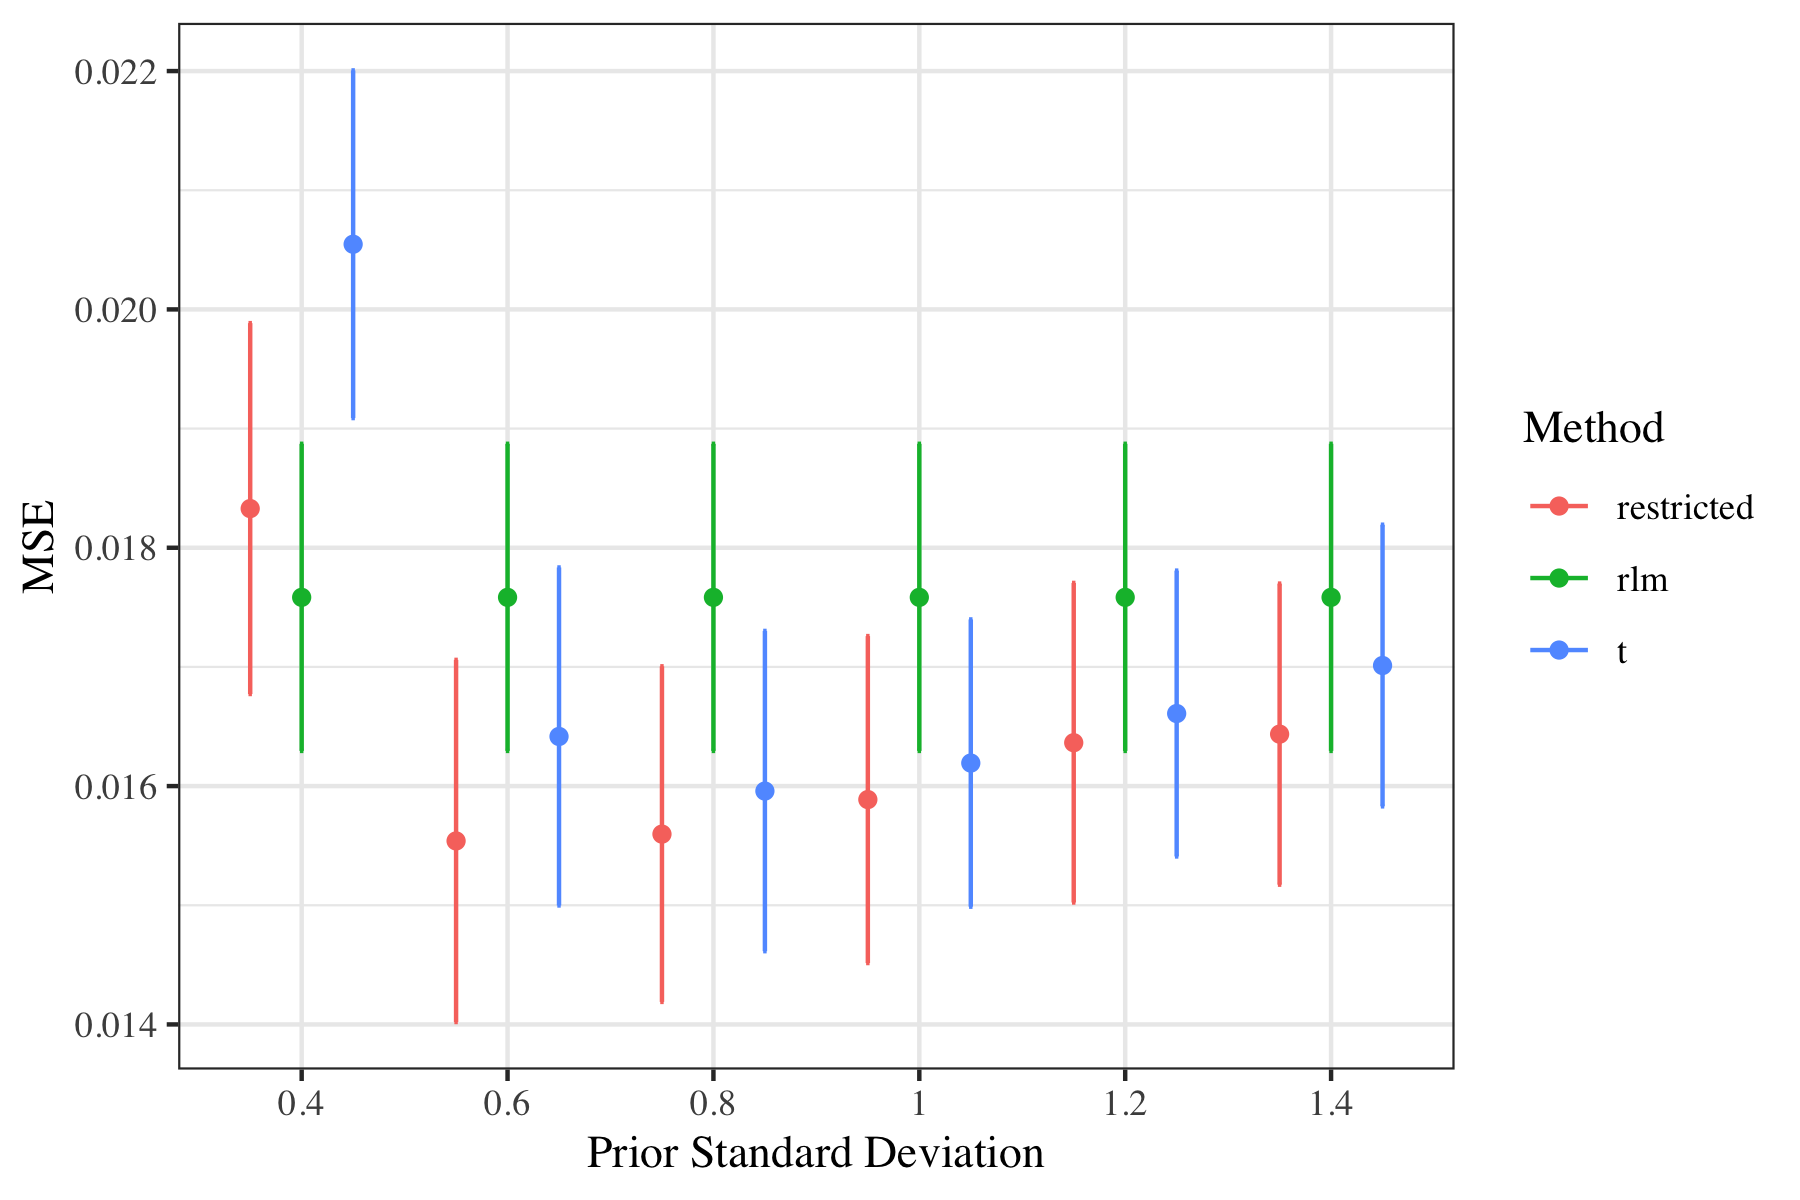
\includegraphics[width = 3.5in]{mse_sim_many_p.png}
%		\caption{Average MSE plus/minus one standard error over the $K = 30$ simulations for each value of the prior standard deviation ($\sigma_{\beta}$) and each of the fitting methods.}
%		\label{mseSimMany}
%	\end{figure}
%\end{frame}
%
%\begin{frame}
%	\frametitle{Prediction of non-outlying data}
%\begin{itemize}
%	\item $MNLL = -\frac{1}{N} \sum \log f(y_{i} |  \hat\bbeta, \hat\bbeta^{*}, \hat\sigma)$, $f$ is the assumed likelihood, average over non-outlying points
%\end{itemize}
%	\begin{figure}[t]
%		\centering
%		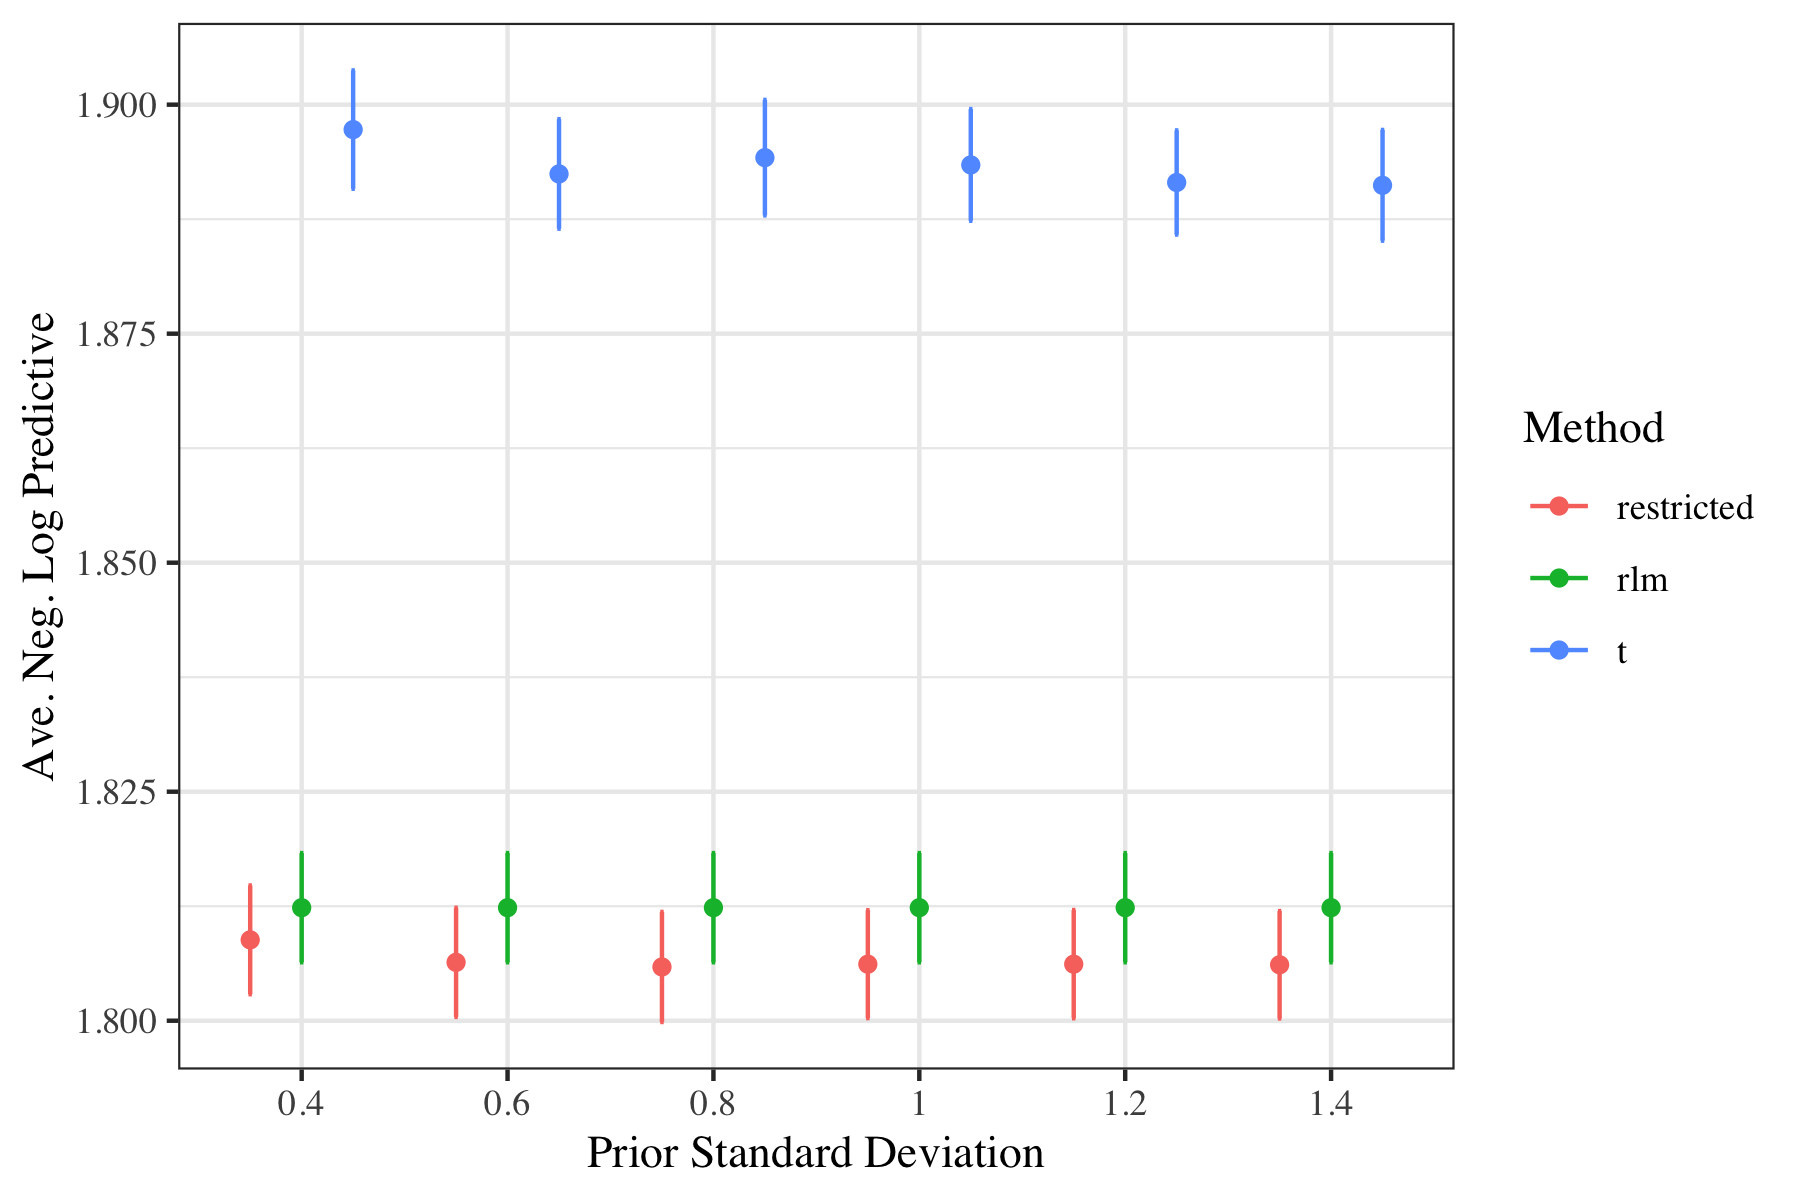
\includegraphics[width = 3.5in]{negll_sim_many_p.png}
%		\caption{Average MNLL plus/minus one standard error for each value of the prior standard deviation ($\sigma_{\beta}$)}
%		\label{negllSimMany}
%	\end{figure}
%\end{frame}
%

\begin{frame}
\frametitle{Real Data: Nationwide Insurance Data}
\begin{itemize}
	\item Nationwide Insurance sells many polices through insurance agencies.
	\item Agencies provide direct service to policy holders.
	\item Contractual agreements between Nationwide and the agencies vary.
	\item Interested in future performance of agencies. 
\end{itemize}
\end{frame}


\begin{frame}
\frametitle{Real Data: Nationwide Insurance Data}
\begin{itemize}
\item Data grouped by states, varying number of agencies by state.
\end{itemize}
	\begin{figure}[t]
		\centering
		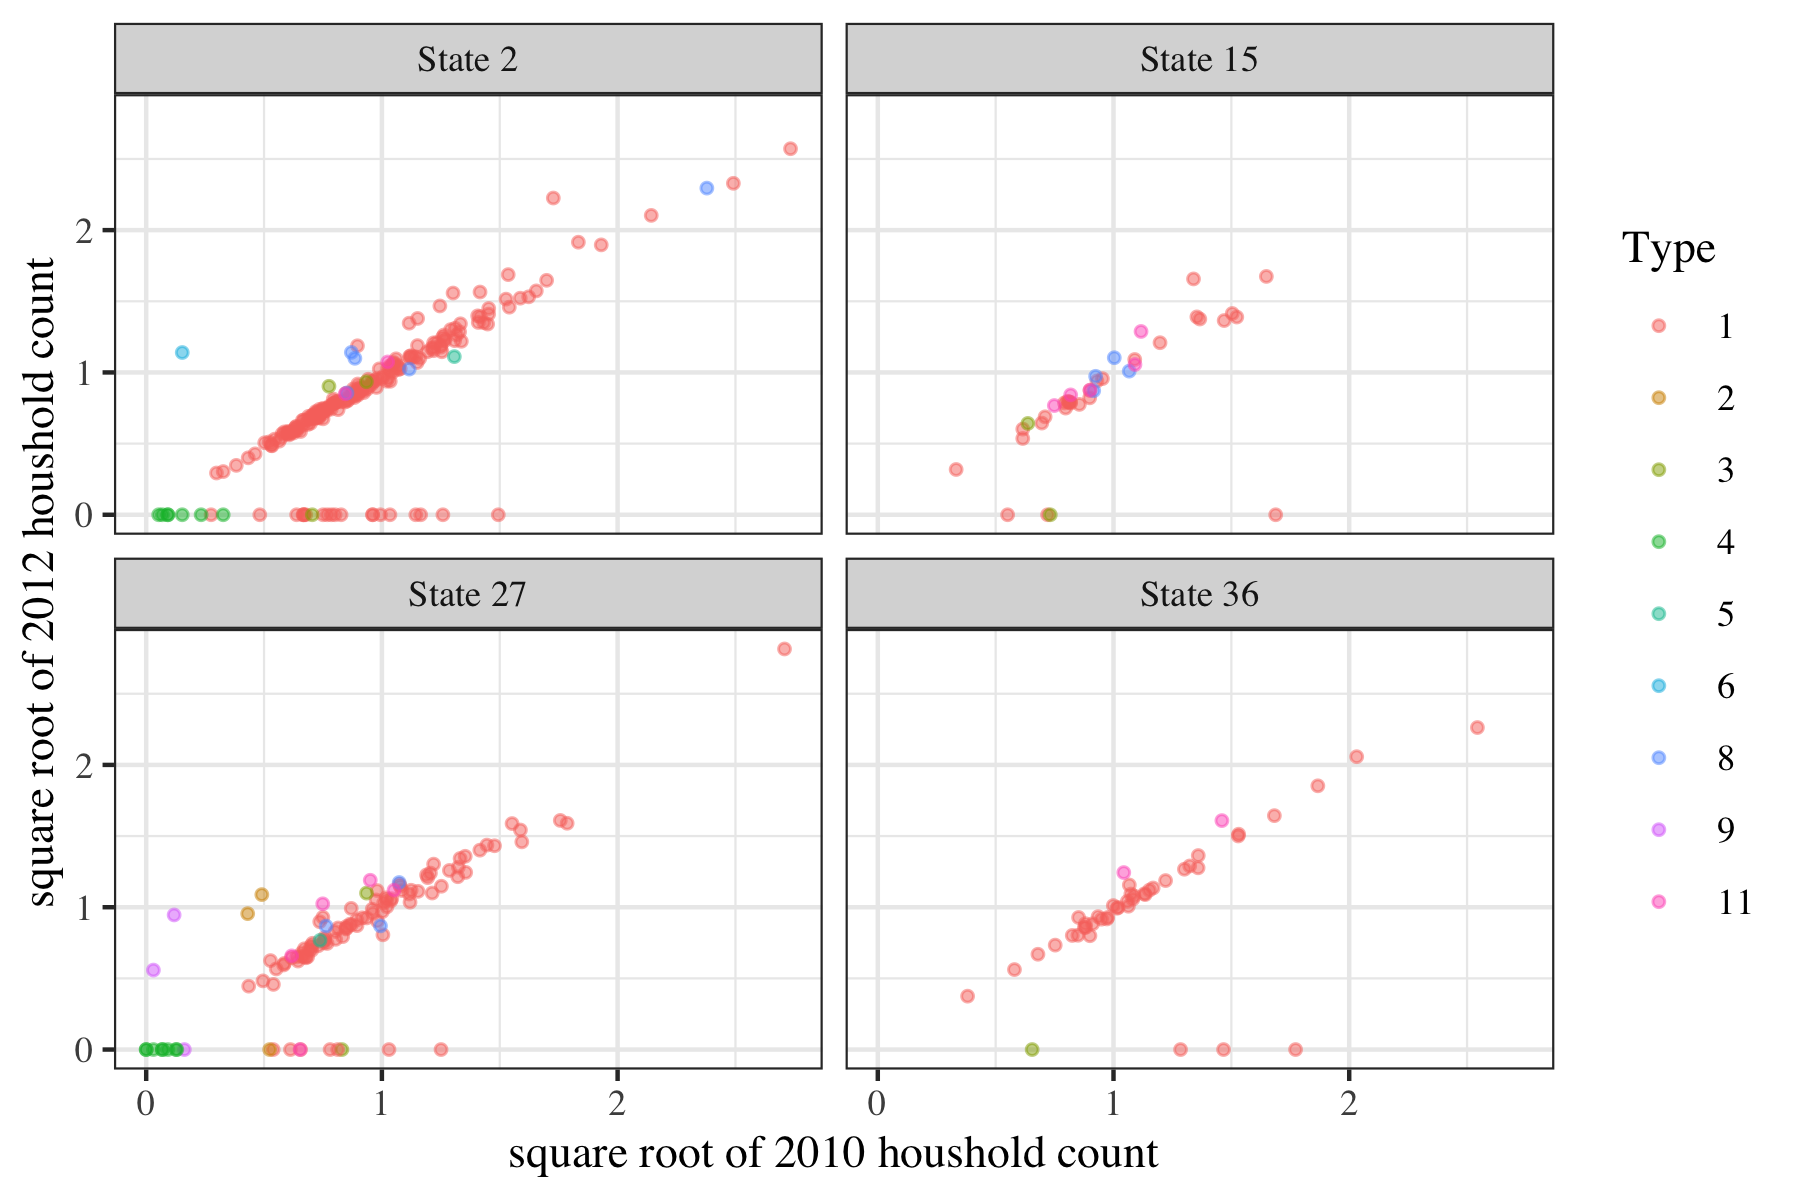
\includegraphics[width=3.5in]{scatter_by_state.png}
		\caption{The square root of (scaled) count in 2012 versus that in 2010 for four states.}
		\label{fig:ctVct}
	\end{figure}
\end{frame}


\begin{frame}
\frametitle{Real Data: State Level Regressions}
Regression fit seperately within each state
\begin{equation*}
\label{eq:regModel}
\bbeta\sim N(\bmu_0, \Sigma_0);\ \ \sigma^2\sim IG(a_0,b_0);\ \  
y_{i}=\bx_{i}^{\top}\bbeta+\epsilon_{i},\ \ \epsilon_{i}\iid N(0, \sigma^2)
\end{equation*}	
\begin{itemize}
	\item Covariates: square root of household count in 2010, two different measures of size and experience.
	\item Response: square root of household count in 2012.
	%\item hyper-parameters fixed via regression of data in time-period two years before. 
	\item model misspecification: omitting contract type, closure information. 
	\item many cases to appear ``outlying" due to misspecification.
\end{itemize}
\end{frame}


\begin{frame}
	\frametitle{Method of Model Comparison}
\begin{itemize}
	\item Both training and validation data will contain outliers
	\item Trimming approach with log predictive density \citep{jung2014}
	\item Case $i$ in holdout set: $log(f(y_i))$
	\item Scoring a procedure:
	\begin{itemize}
		\item Choose a base method (e.g. Student-t model) and trimming fractions $\alpha$
		\item Order holdout sample by $log(f_b(y_i))$
		\item Denote ordering by: $y_{(1)}^b, y_{(2)}^b, \dots, y_{(M)}^b$
		\item score each method with ``mean trimmed log margainal psuedo likelihood"
	\end{itemize}
\[TLM_b(A) = (M - [\alpha M])^{-1} \sum_{i=[\alpha M]+1}^{M}
\log(f_A(y_{(i)}^b)),\]
\end{itemize}
\begin{itemize}
	\item $f_A$ - predictive distribution under the method ``A'' being scored. 
\end{itemize}
\end{frame}


\begin{frame}
	\frametitle{Predictive Performance: 50 training/holdouts sets}
Evaluation of `Type 1' agencies (of special interest to the company)
\begin{figure}[t]
	\centering
	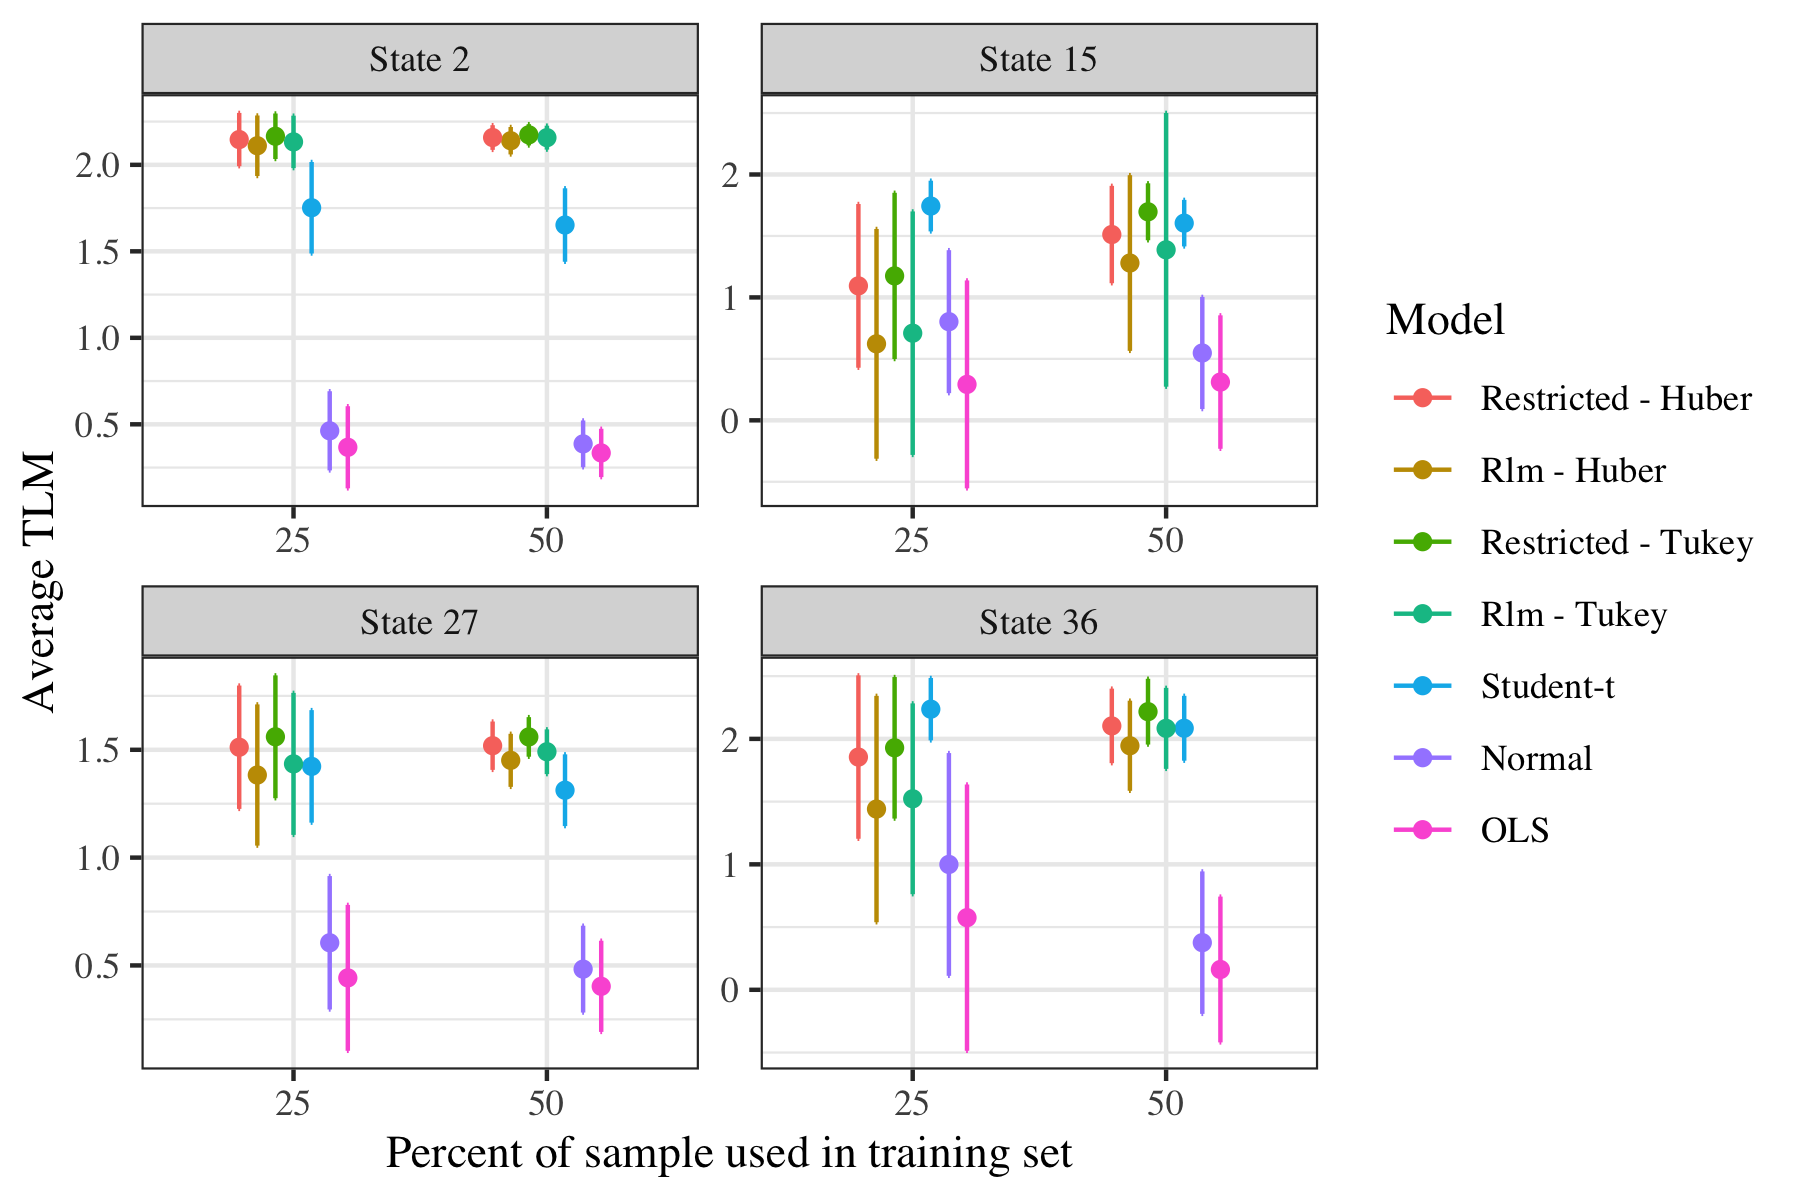
\includegraphics[width=4in]{tlm_base_Student-t.png}
	\caption{$\alpha = 0.3$. States 2, 15, 27, and 36, have $n = 222, 40, 117,$ and $46$}
	\label{fig:tlm}
\end{figure}
\end{frame}

\begin{frame}
	\frametitle{Predictive Performance}
\begin{itemize}
\item Normal Theory/OLS perform poorly due to not accounting for misspecification
\item Small, consistent improvement over classical methods
\item variance reduction 
\item diminishing of effect of prior - similar performance in larger states. 
\item heavy-tailed model performs worse in the larger states - more outliers appear. 
\end{itemize}
	
\end{frame}


%\begin{frame}
%	\frametitle{Predictive Performance: changing trimming fraction}
%	
%\begin{figure}[t]
%	\centering
%	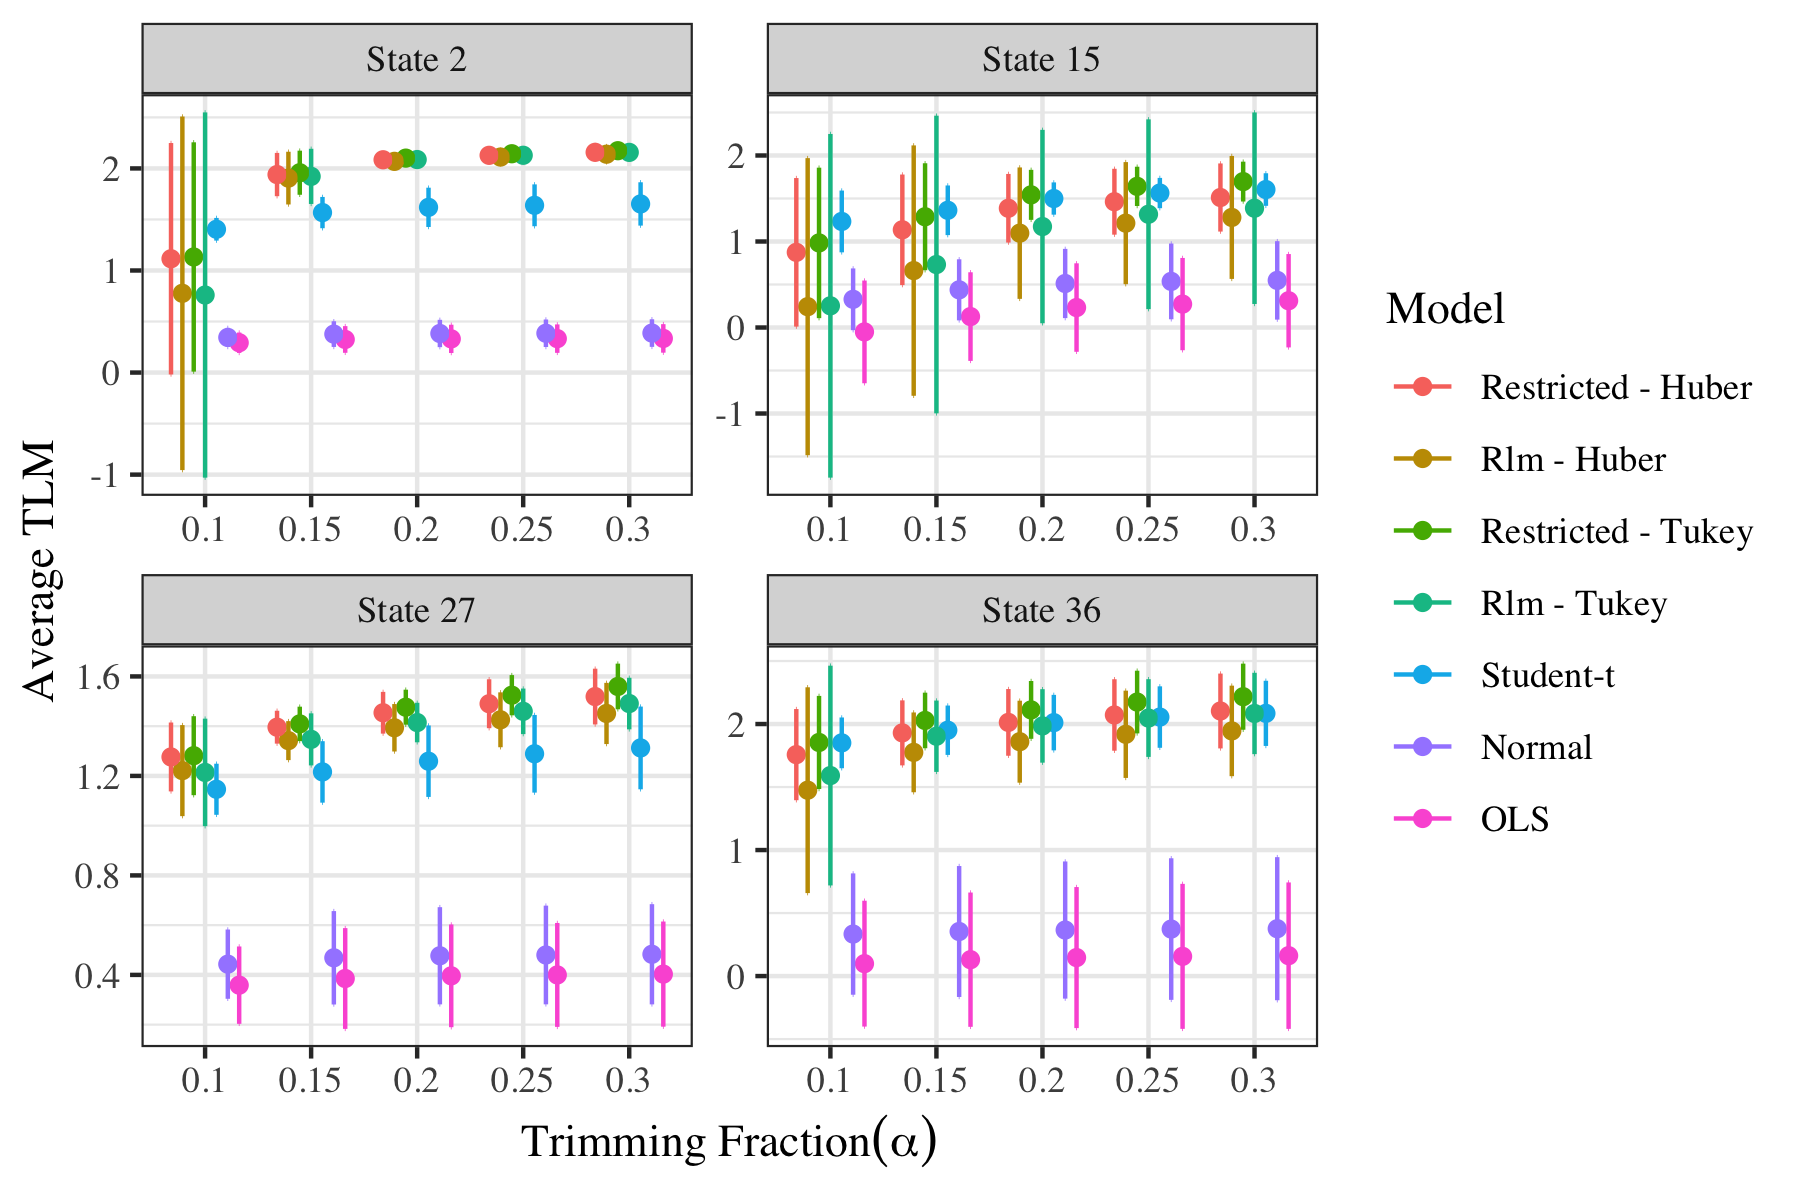
\includegraphics[width=4.5in]{tlm_base_Student-tbyTrimming.png}
%	\label{fig:tlmbyAlpha}
%\end{figure}
%
%	
%\end{frame}


\begin{frame}
\frametitle{Real Data: Hierarchical Regression}
\begin{align*}
%\begin{split}
\label{eq:hierModel}
&\bbeta\sim N_p(\bmu_0, a\Sigma_0);\ \ 
\bbeta_j\iid N_p(\bbeta, b\Sigma_0); \ \  
\sigma_j^2\sim IG(a_0,b_0);  & \\ 
& y_{ij}=\bx_{ij}^\top\bbeta_j+\epsilon_{ij},\ \ \epsilon_{ij}\iid N(0, \sigma_j^2),\ i=1,\dots, n_j,\ j=1,\dots, J &
%\end{split}
\end{align*}	
\end{frame}

\begin{frame}
	\frametitle{Predictive Performance}
Average of State-level performance $\overline{TLM}_b(A)_{\cdot}= \frac{1}{J} \sum_{j =1}^{J} TLM_b(A)_{j}$
\begin{figure}[t]
	\centering
	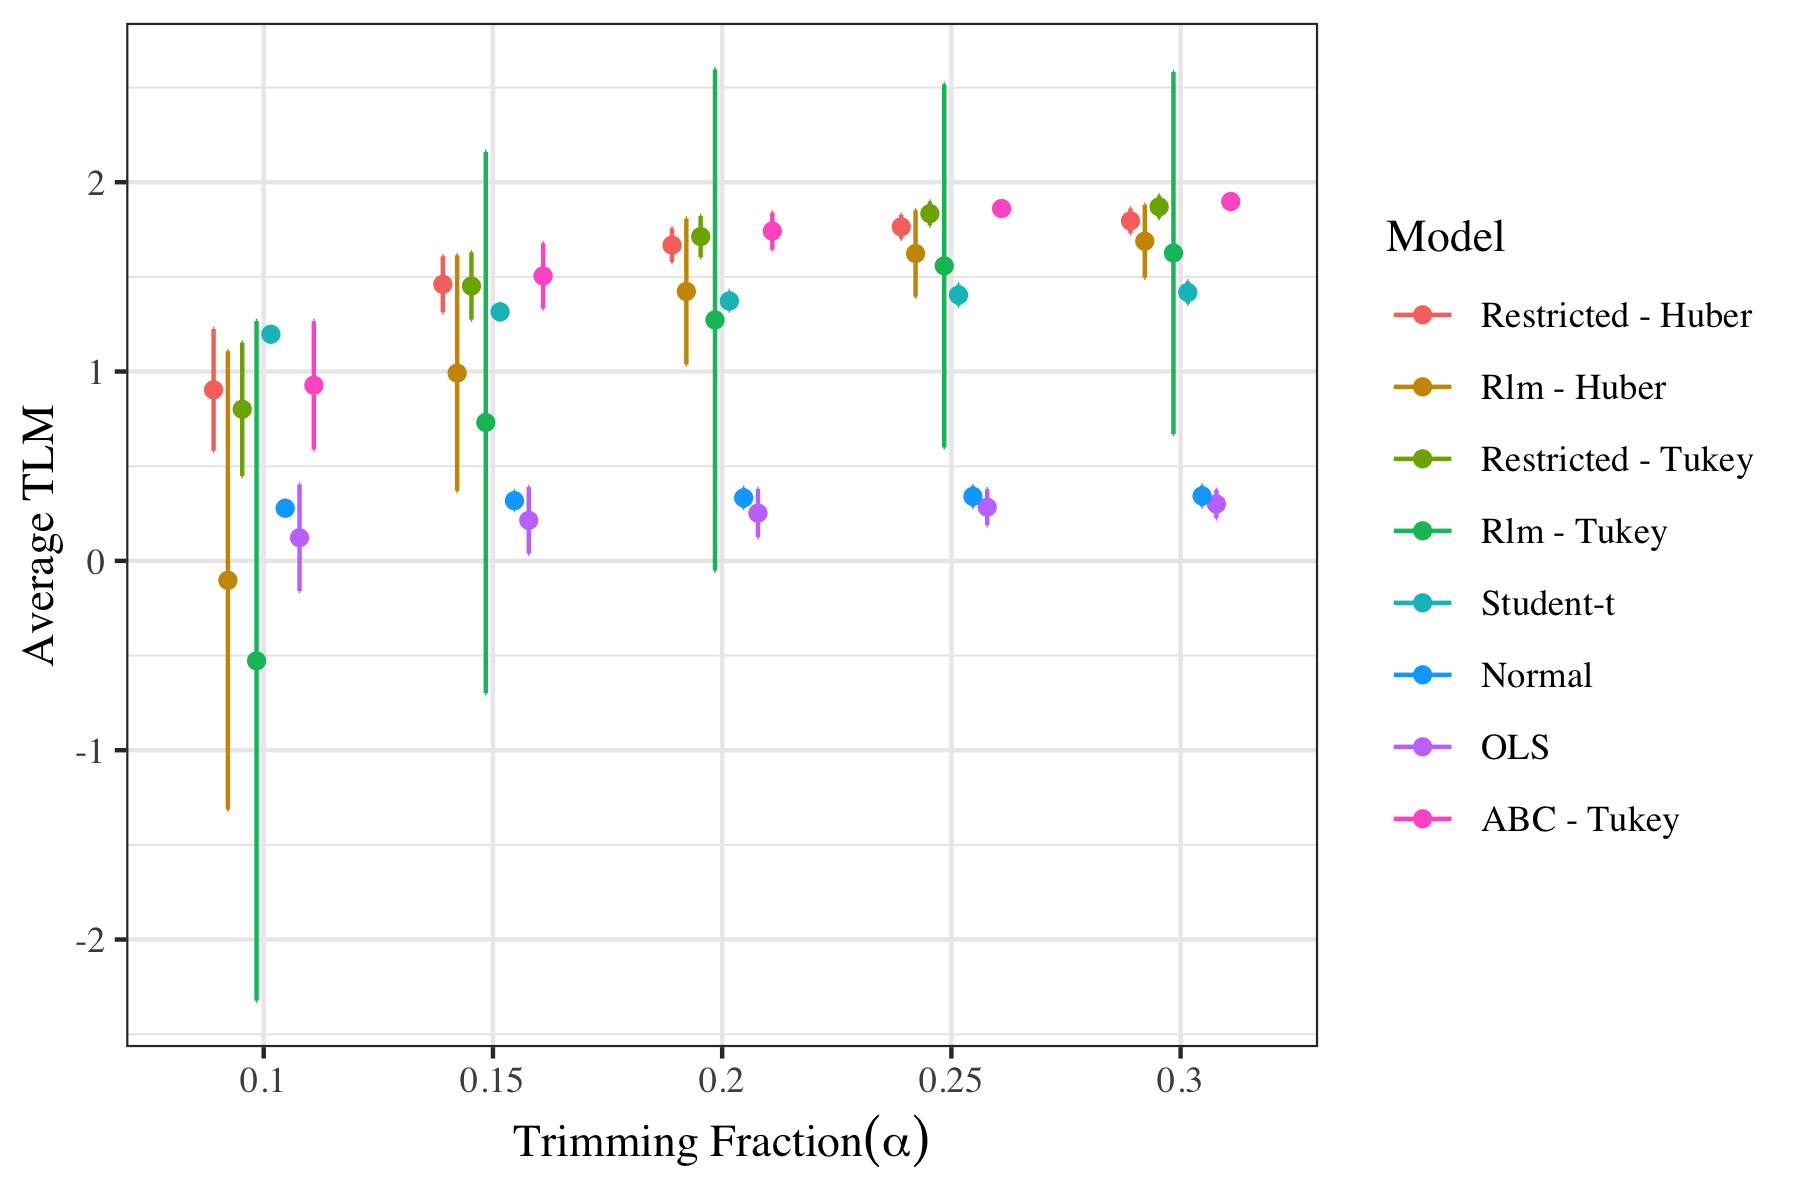
\includegraphics[width=4.25in]{hier_average_tlm.png}
	\label{fig:hierTLM}
\end{figure}
\end{frame}


\begin{frame}
	\frametitle{Predictive Performance - Notes}
\begin{itemize}
\item t-model's poorer performance attributed to the heavier tails - no natural mechanism for prediction. 
\item Bayesian versions outperform classical robust counterparts. Also reduction in variance. 
\item ABC also performs well - perhaps better, but this can be attributed to a single state. 
\end{itemize}
	
\end{frame}



\begin{frame}
	\frametitle{Predictive Performance by State}
\begin{itemize}
	\item restricted likelihood average TLM is larger than ABC in 14 of the 20 states, median difference of $0.04$
\end{itemize}
\begin{figure}[t]
	\centering
	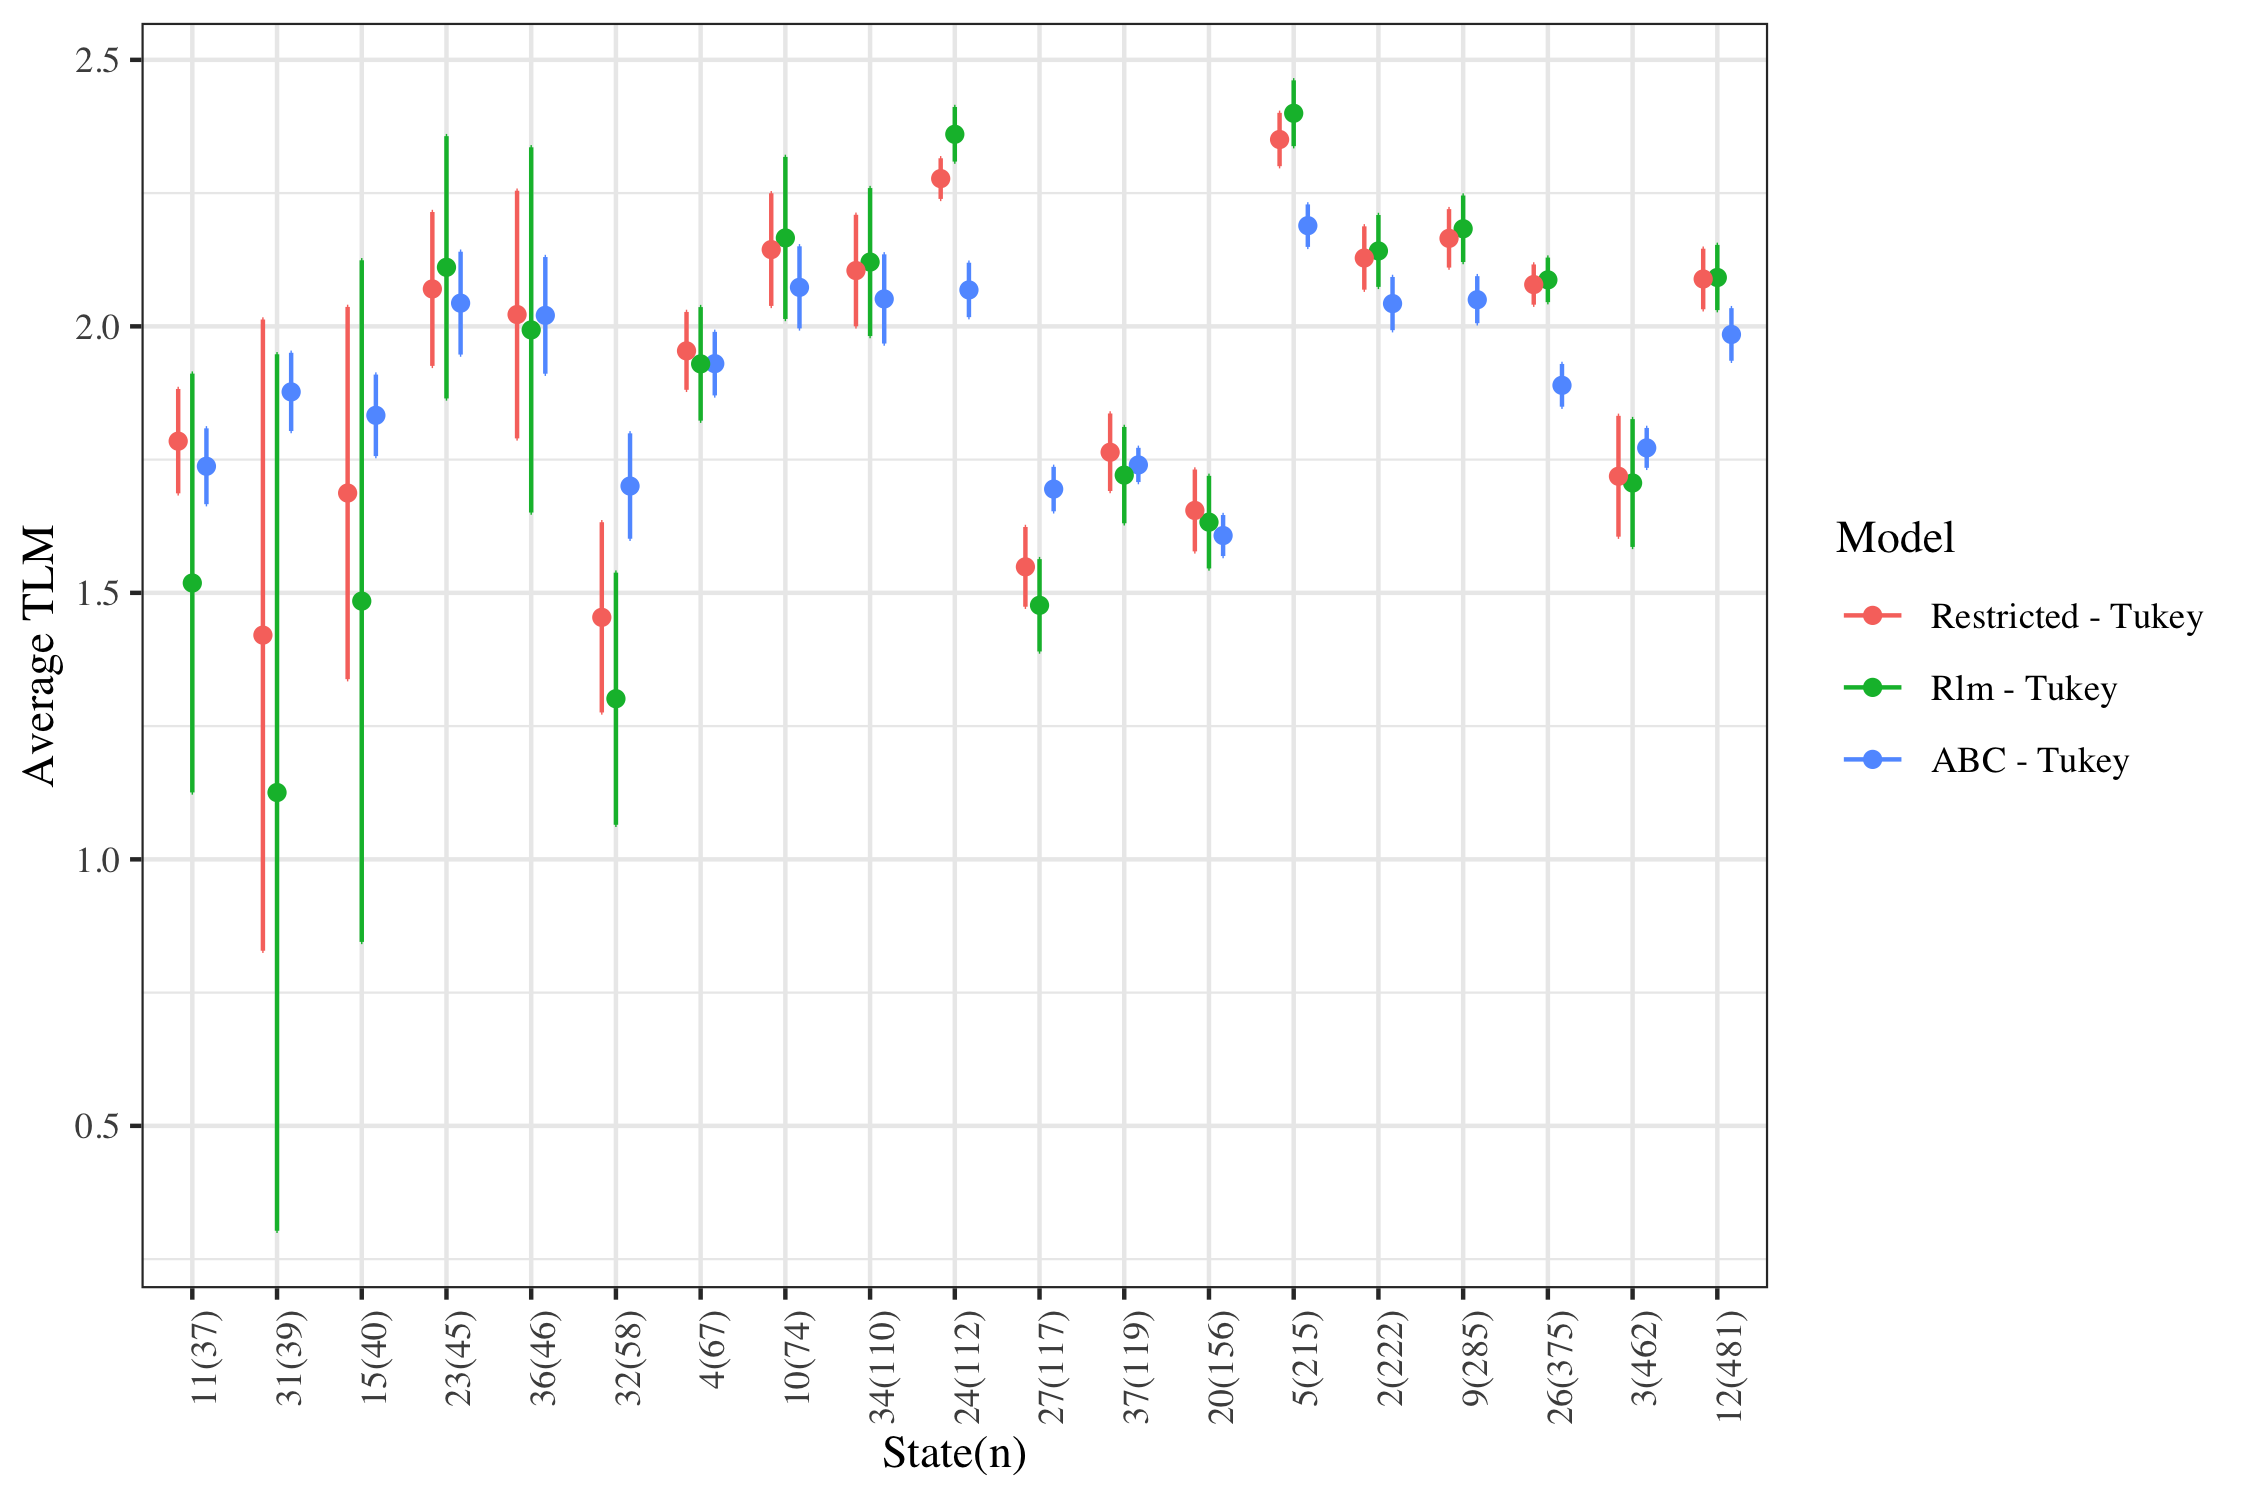
\includegraphics[width=4.25in]{hier_ave_tlm_state.png}
	\label{fig:hierTLM}
\end{figure}

\end{frame}


\begin{frame}
	\frametitle{Predictive Performance by State - Notes}
\begin{itemize}
\item Our method tends to perform well in the smaller states in comparison to classical counter part
\item Similar performance in larger states - as expected
\item Better than ABC in 14/20 states. Better overall performance of ABC attributed to a single state (31). 

\end{itemize}
	
\end{frame}



%\begin{frame}[t,allowframebreaks]
%	\frametitle{References}
%	\def\newblock{\hskip .11em plus .33em minus .07em} % important line
%	\bibliography{bib/refPaper1.bib}
%\end{frame}
	
\end{document}